\documentclass[conference]{IEEEtran}
\IEEEoverridecommandlockouts
% The preceding line is only needed to identify funding in the first footnote. If that is unneeded, please comment it out.
\usepackage[utf8]{inputenc}
\usepackage[T1]{fontenc}
%\usepackage[ngerman]{babel}
\usepackage{cite}
\usepackage{amsmath,amssymb,amsfonts}
\usepackage{algorithmic}
\usepackage{graphicx}
\usepackage{textcomp}
\usepackage{xcolor}
\usepackage{hyperref}
\usepackage{cleveref}
\usepackage{xcolor}
\usepackage{float}
\hypersetup{
	colorlinks   = true, %Colours links instead of ugly boxes
	urlcolor     = blue, %Colour for external hyperlinks
	linkcolor    = blue, %Colour of internal links
	citecolor   = black %Colour of citations
	%hidelinks = True
}
\def\BibTeX{{\rm B\kern-.05em{\sc i\kern-.025em b}\kern-.08em
    T\kern-.1667em\lower.7ex\hbox{E}\kern-.125emX}}
\newcommand{\figPath}{images}

\begin{document}

\title{Examination paper for software laboratory pandapower}

\author{\IEEEauthorblockN{Dennis Weispfennig}
\IEEEauthorblockA{\textit{e\textsuperscript{2}n Energy Management} \\
\textit{and Power System Operation}\\
\textit{University Kassel}\\
Kassel, Germany \\
\href{mailto:uk061572@student.uni-kassel.de}{uk061572@student.uni-kassel.de}}
%\and
%\IEEEauthorblockN{2\textsuperscript{nd} Given Name Surname}
%\IEEEauthorblockA{\textit{dept. name of organization (of Aff.)} \\
%\textit{name of organization (of Aff.)}\\
%City, Country \\
%email address or ORCID}
%\and
%\IEEEauthorblockN{3\textsuperscript{rd} Given Name Surname}
%\IEEEauthorblockA{\textit{dept. name of organization (of Aff.)} \\
%\textit{name of organization (of Aff.)}\\
%City, Country \\
%email address or ORCID}
%\and
%\IEEEauthorblockN{4\textsuperscript{th} Given Name Surname}
%\IEEEauthorblockA{\textit{dept. name of organization (of Aff.)} \\
%\textit{name of organization (of Aff.)}\\
%City, Country \\
%email address or ORCID}
%\and
%\IEEEauthorblockN{5\textsuperscript{th} Given Name Surname}
%\IEEEauthorblockA{\textit{dept. name of organization (of Aff.)} \\
%\textit{name of organization (of Aff.)}\\
%City, Country \\
%email address or ORCID}
%\and
%\IEEEauthorblockN{6\textsuperscript{th} Given Name Surname}
%\IEEEauthorblockA{\textit{dept. name of organization (of Aff.)} \\
%\textit{name of organization (of Aff.)}\\
%City, Country \\
%email address or ORCID}
}

\maketitle

\begin{abstract}
For the seminar on the use of pandapower a example grid is provided and a time series for the load and generation was given. The results of the time series calculation shows some voltage violations and line overloading at specific times. Those violations are then corrected trough the use of controllers in the pandapower framework. After the controllers are set up and used in the time series calculation the voltage violations and line overloading in the designated subgrid are eliminated.
\end{abstract}

\begin{IEEEkeywords}
pandapower, electrical grid, time series, controller, seminar
\end{IEEEkeywords}

\section{Introduction \& Examination task description}
Throughout the seminar we learned to use the pandapower module in python to run power flow calculations an electrical distribution and transmission grids.\cite{pandapower.2018} To show that we understood how to use the pandapower module to solve a grid planing problem a example grid is provided with a corresponding time series of the load and generation power as a series of scaling factors that are applied to the nominal installed power of all loads and generators in the grid. As the examination task we are asked to select one of the four subgrids at random and then analyze it for voltage violations were the node voltage is lower then 0.95 p.u. or higher then 1.05 p.u. and overloaded lines where the line loading is above 100\%. After the subgrid is analyzed and all violations are recorded, we are tasked to develop a controller that runs within the time series calculation and adjusts parameters in the subgrid to prevent voltages or line loadings from breaching the limits. If the developed controller is able to prevent the violation of limits in the selected subgrid, we are tasked to import a controller that works on another subgrid that is different from the one we selected and implement this one in our code. After the implementation we are tasked to make sure that our controller is not disturbed by the new controller and still prevents the violation of limits in our subgrid. 

\section{Analyzing the chosen subgrid}

\begin{figure}[t]
	\centering
	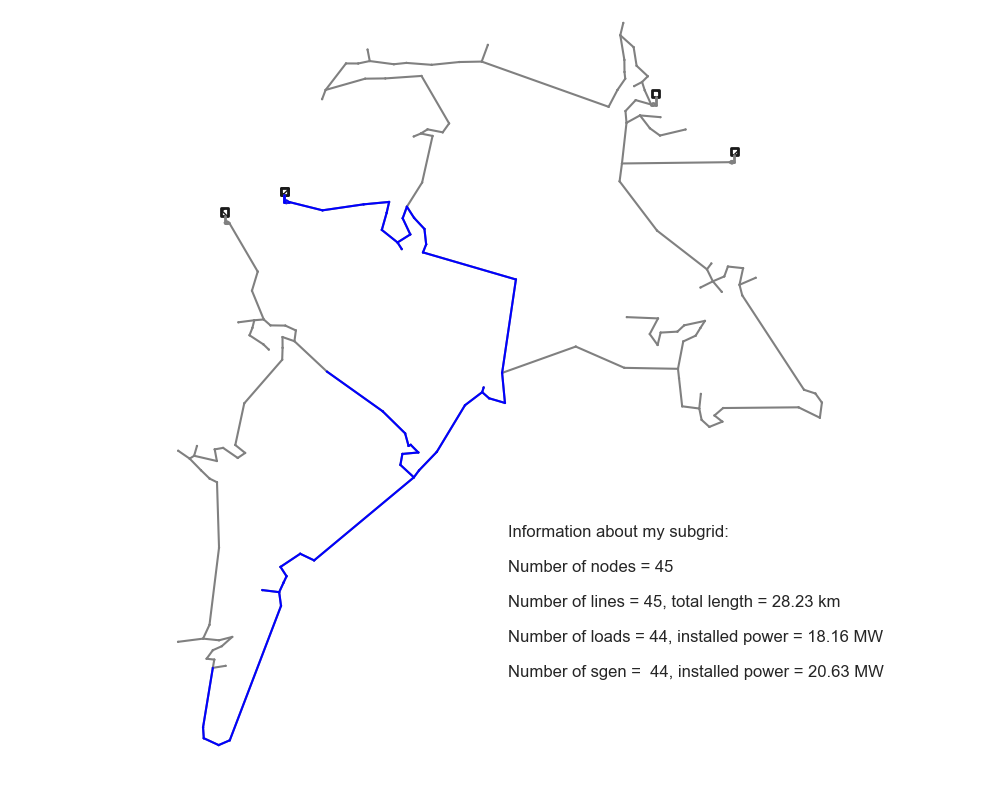
\includegraphics[width=\linewidth]{\figPath/Task_1_colored_grid.png}
	\caption{Overview of the whole grid with my subgrid highlighted in \textcolor{blue}{blue}}
	\label{fig:grid_overview}
\end{figure}

For this examination I chose the subgrid number 2 from the slide 62 from the presentation that accompanies this software laboratory.\cite[S.62]{software.lab.pp.2023} In my chosen subgrid are in total 45 nodes, with 45 lines. The total line length is 28.23 km and in the subgrid are 44 loads and 44 static generators installed. All loads combined posses a nominal power of 18,16 MW and all static generators combined posses an installed nominal generation capacity of 20.63 MW. After running the given time series scaling factors for the loads and static generators the results show voltage violations and overloaded lines. To illustrate the power flow results the minimum and maximum p.u. voltage over all 45 nodes as well as the maximum line loading in my subgrid are logged and then plotted in \cref{fig:pf_res_task_2}. The highest calculated voltage in my subgrid was 1.08 p.u. and the lowest calculated voltage was 0.91 p.u. in total 30,8\% of all time steps show a violation of the voltage limits. In 20,68\% of the calculations the voltage at one bus was higher then 1.05 p.u. and in 10,12\% the voltage was bellow 0.95 p.u. the line loading is comparison not so prominent. Only in 0.89\% of all time step calculations was the limit of 100\% line loading exceeded. The highest line loading calculated was 111,52\%.

\begin{figure*}[htbp]
	\centering
	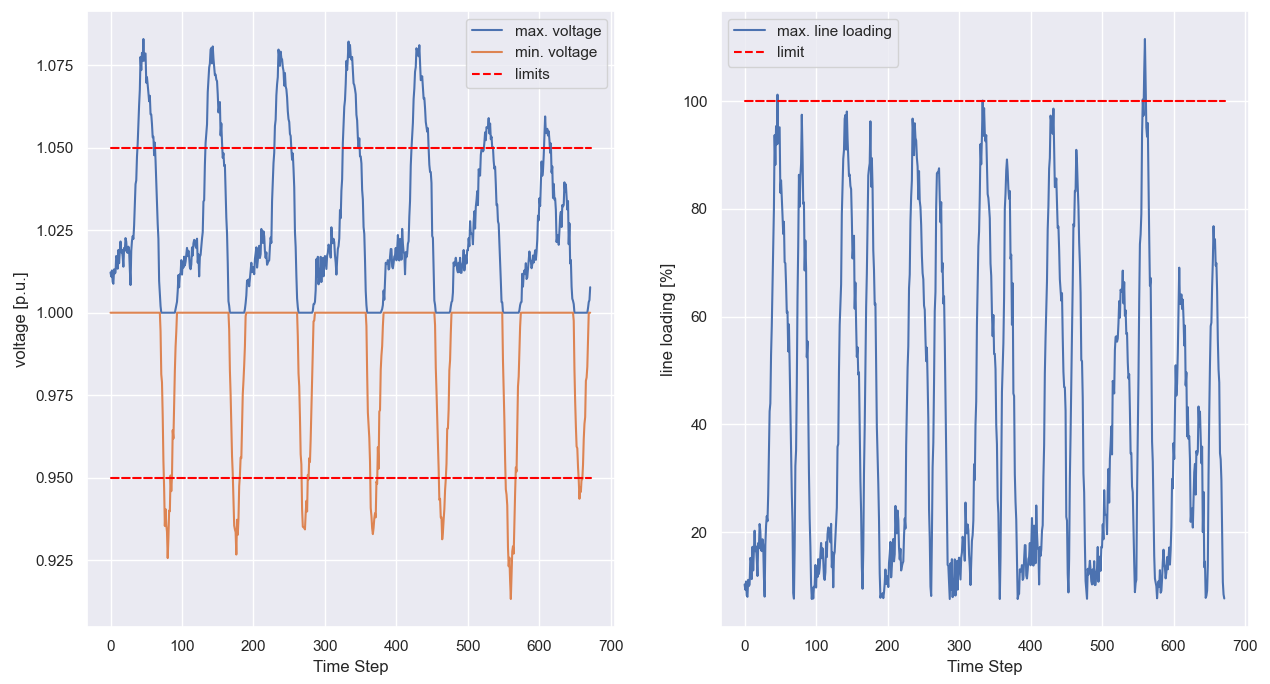
\includegraphics[width=\linewidth]{\figPath/Task_2_subgrid_results.png}
	\caption{Power flow results from the time series calculation}
	\label{fig:pf_res_task_2}
\end{figure*}

\section{Consideration on the type controller to use}

The pandapower module provides two general types of controllers. 
\begin{itemize}
	\item Central controllers
	\item Local controllers
\end{itemize}
\subsection{Local controllers}
A local controller is used to specifically control one element and do not affect other elements in the grid. These controllers take the calculation results for the specified element and adjust parameters of this element in accordance with the results and the behavior the controller is designed to present.
\subsection{Central controllers}
Another type of controller is the central controller, that monitor all results from the whole grid and affect more then one element of the whole grid at a time.
\subsection{Deciding on a controller type}
In order to prevent the voltage and line loading from violation the limits I decided to use a central controller, that affects all loads and generators in my subgrid together. My controller is designed to operate in two different modes. 
\begin{figure*}[htbp]
	\centering
	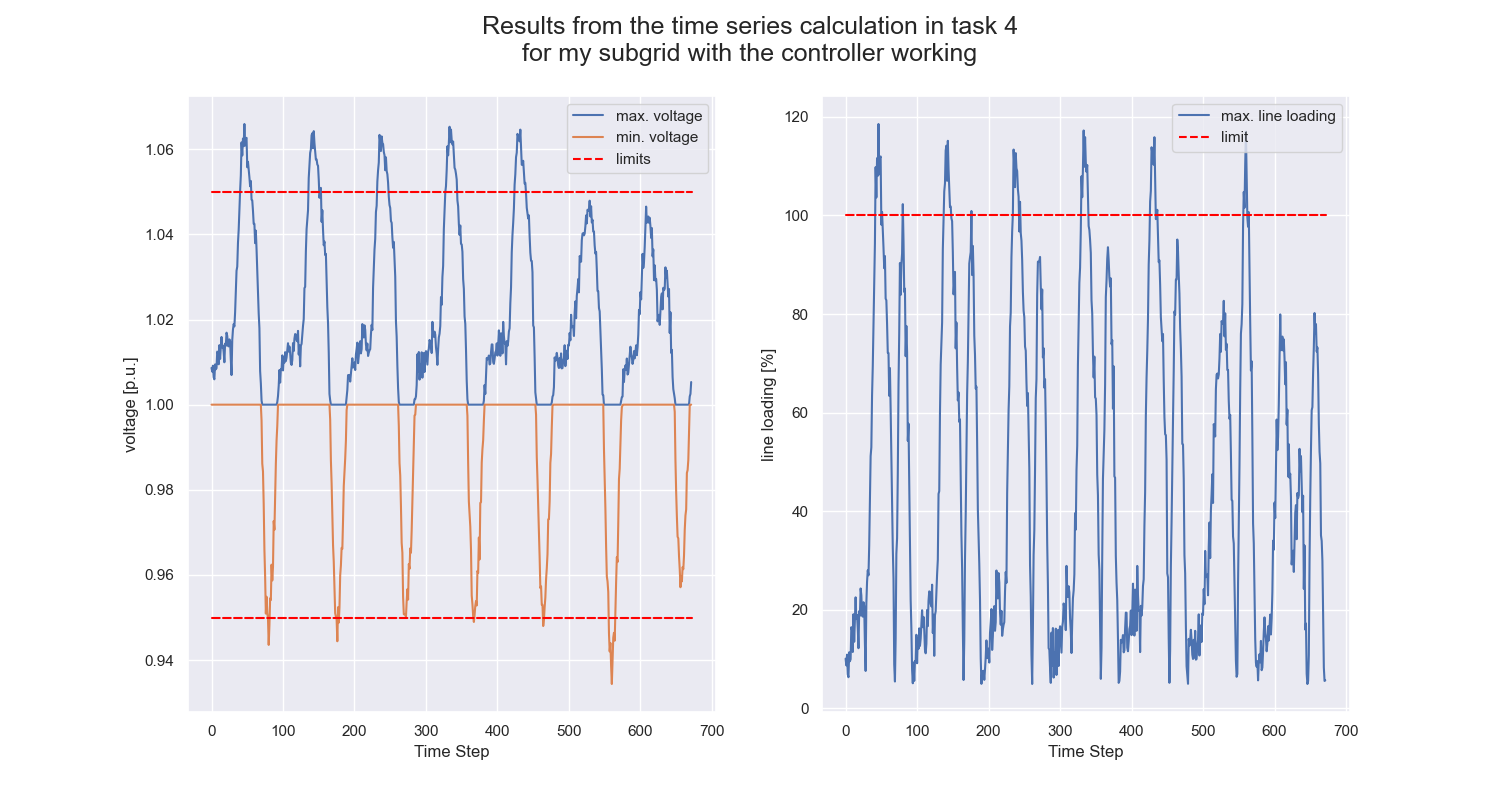
\includegraphics[width=\linewidth]{\figPath/Task_4_subgrid_results.png}
	\caption{Power flow results from the time series calculation with the controller working}
	\label{fig:pf_res_task_4}
\end{figure*}
\begin{figure*}[htbp]
	\centering
	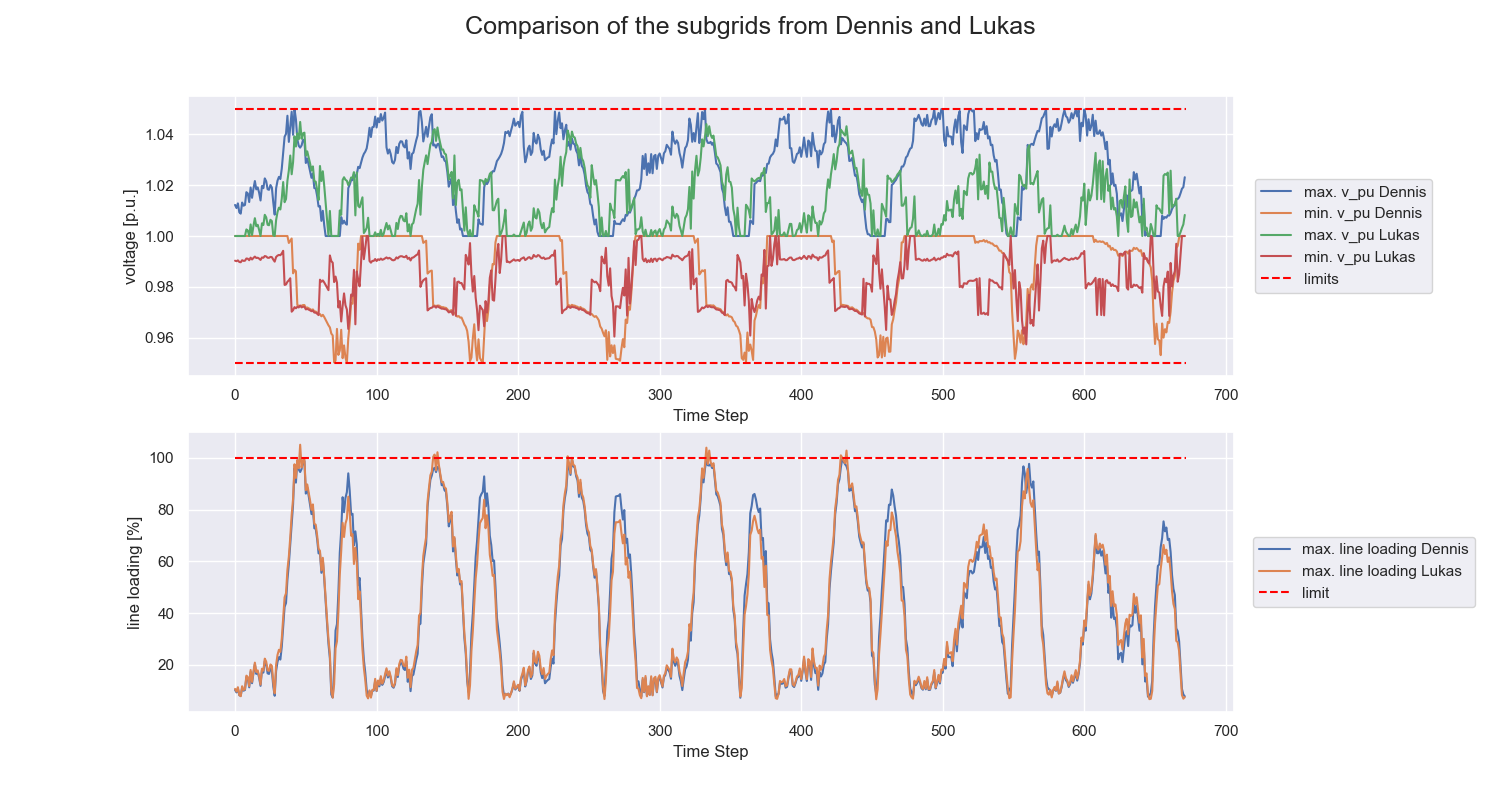
\includegraphics[width=\linewidth]{\figPath/comp_res_dennis_lukas.png}
	\caption{Comparison of the time series calculation results of my and Lukas subgrids with working controllers in both subgrids}
	\label{fig:pf_res_task_5}
\end{figure*}
\subsection*{Voltage control}
The first mode is \textit{voltage} mode in which the controller first tries to adjust the tap position of the transformers in the grid. If the maximum voltage in the subgrid is above the upper limit of 1.05 p.u. the tap position of the transformer is increased to lower the output voltage and check if this action solved the violation. Similarly the tap position is increase, if the minimum voltage in the subgrid is below the lower limit. Should the tap position reach the lowest/highest setting and the voltage violation is still present, then the controller internally switches to the line loading setting, because this setting adjusts the scaling factor of the loads and generators. But the convergence check is still done on the voltage limits and not the line loading.
\subsection*{Line loading control}
The second mode \textit{line\_loading} is designed to prevent the line loading from violation the limit. To achieve this task the controller first checks if a line in the subgrid exceeds the loading limit and then calculates if the overload is most probably caused by an excess of load demand of generation power. To do this the real power result of the slack is selected and if it is positive it's assumed that a excess of load demand is causing the overload. Then the current scaling factor ($\text{f}_{\text{p,i}}$) of of all loads in the subgrid is multiplied by 0.9 to reduce the scaling factor for the next iteration ($\text{f}_{\text{p,i+1}}$) a tiny bit until the overload disappears.
\begin{equation}
	\text{f}_{\text{p,i+1}} = \text{f}_{\text{p,i}} \cdot 0.9
\end{equation}

In the case where the real power value of the slack is negative a excess of generation could be the problem and in this situation the loads in the subgrid are used to reduce the line loading. This is done in this case, because I assume that the load can be increased at will, but the generation in the previous case is at its maximum and so can't reduce the load by increasing its generation. The scaling factor for the loads in this case is increased in each iteration until the overload of the lines disappears. 
\begin{equation}
	\text{f}_{\text{p,i+1}} = \text{f}_{\text{p,i}} \cdot 1.1
\end{equation}

Or until the scaling factor reaches 1.0 and then the scaling factor for the generation is decreased in each iteration as it is done to the load scaling factor. Should the reactive power at the slack exceed the real power, then both loads and generators are scaled down by the controller, because the implementation of the reactive power control would depend on the nominal apparent power and the reactive power limits of each element in the subgrid.
\subsection{Results}
After designing the controller and implementing it in the \textit{voltage} and \textit{line\_loading} mode, all violations are eliminated. Because the controller takes the subgrid as an input, the actions of it are limited to only the subgrid and the violations in the other subgrids occur regardless. The results are shown in \cref{fig:pf_res_task_4}. The limits for the voltage level and line loading is reached but never violated.
\subsection{Interaction with multiple controllers}
If more then one controller are present in a grid it is possible that those controllers interfere with each other. In pandapower each controller has a \textit{level} and \textit{order} that determine when each controller is executed. Controller with the same level are executed in series and are both required to converge in the same iteration. The higher the level of a controller the later it is run and so can overwrite the results of controllers in lower levels. This means that a controller in level 0 that previously converged might not be satisfied after the last controller in the highest level converged.
\subsection*{Merging of different Git-Branches}
To show, that the version control tool Git and the extension GitHub for distributed version control and collaboration is used during the software laboratory a controller from another student is implemented in my branch of the pandapower GitHub repository. I chose the controller from Lukas Kramer and implemented it into my script and ran another time series calculation to see, if my controller still operates as expected. In \cref{fig:pf_res_task_5} the maximum/minimum voltages and maximum line loading of my and Lukas subgrids are plotted and it shows, that my controller still works in my subgrid and Lukas controller works in his subgrid to prevent voltage violations. Lukas controller was not designed to prevent overloaded lines and so works as expected in his subgrid. 
\bibliography{my_bib} 
\bibliographystyle{ieeetr}

\end{document}
